\Author{\daAuthorOne}
% \usepackage[backend=biber, style=alphabetic]{biblatex}

The Admin Panel is a centralized administrative dashboard to efficiently manage all addresses within a single environment. It is used to plan for future "Sternsinger" events, ensuring that every address that needs to be visited is covered and that all addresses are efficiently distributed among participating groups. Additionally, it enables the assignment of areas containing addresses a group needs to visit. This zoning feature ensures that each group is responsible for visiting only the addresses within their assigned area.\\

With the tool, administrators can perform CRUD (Create, Read, Update, Delete) operations on addresses, streets, and areas. These features make it easy to quickly address issues and make changes to the areas that participants need to visit. For example, if a new street is added to the neighborhood, the administrator can update the system to include this street and assign it to the appropriate area. Similarly, if a group drops out, the administrator can quickly reassign the addresses that have not yet been visited to other groups. This ensures that the data remains up-to-date and allows for quick reactions to special cases, helping with the planning and execution of "Sternsinger" events.\\

This chapter will outline the implementation of the Admin Panel and describe the different components, functionalities, and widgets of this tool. Additionally, it will provide information on how to use it.\\\\

\subsection{Navigation}

\begin{figure}[H]

\begin{minipage}{0.58\textwidth}
    \setstretch{1.5} % Erhöht den Zeilenabstand
    To navigate between pages, a sidebar on the left is used, which can be toggled with a button in the top-left corner of the screen. It shows a list of all pages, allowing users to switch between them with a click.

    The navigation is implemented in the file \texttt{AdminNavigation}. It contains a list of pages with titles. These titles are displayed at the top of the screen above the corresponding page. To keep track of the currently selected page, an internal state (\texttt{indexState}) is used. Whenever a page is selected in the sidebar, the \texttt{indexState} is updated, and the corresponding page is displayed. This widget is the main component. It makes sure that all pages are properly displayed.
    \end{minipage}
    \hfill
    \begin{minipage}{0.38\textwidth}
    \centering
    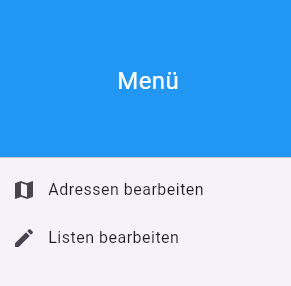
\includegraphics[width=\linewidth]{images/AdminPanel/Menu.png}
    \caption{Navigation in Admin-Panel}
    \label{fig:adminpanel_navigation}
\end{minipage}

\end{figure}

%Zeilenumbruch um neue Seite zu starten
\newpage

\begin{subsection}{AddressPage}
    \sloppy
    The first page, the \texttt{AddressPage}, displays an interface to create, update, and delete address data. It uses a form with various input fields (e.g., street, house number, coordinates, special features) and a map or database view to visualize and select addresses. The page is divided into two parts:

    \begin{itemize}
        \item On the right side, all addresses are shown either in the \texttt{AdminMapComponent} (\ref{fig:AdminMapComponent}) or the \texttt{DatabaseViewComponent} (\ref{fig:DatabaseViewComponent}). These two components display the same addresses but in different ways, to give the administrator the choice of how they want to view the addresses.
        \item On the left side of the page are \texttt{InputFields} (\ref{fig:InputField}), which are used to enter new information about a new address or edit an existing one.
    \end{itemize}

    Overlaying the \texttt{AdminMapComponent}, there are:

    \begin{itemize}
        \item A field to filter the addresses displayed.
        \item A button with a dropdown menu to select and edit a street.
        \item A switch to toggle between the \texttt{AdminMapComponent} and the \texttt{DatabaseViewComponent}.
        \item An information box in the bottom left corner to display \texttt{Notifications} (\ref{fig:Notification}) about the completed operations.
        \item A field in the bottom right corner to display the coordinates of the mouse pointer on the map.
    \end{itemize}
    

    \begin{figure}[H]
        \centering
        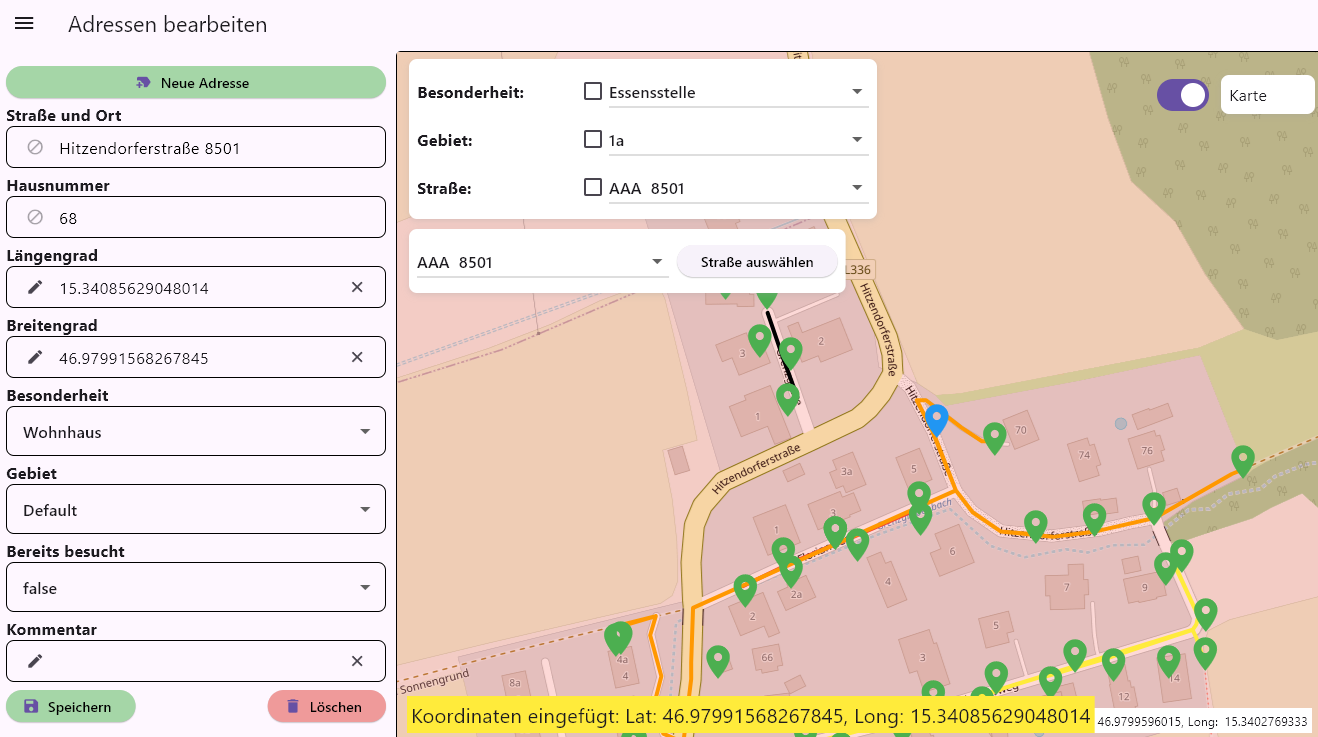
\includegraphics[width=1\linewidth]{images/AdminPanel/AddressPage.png}
        \caption{AddressPage}
    \end{figure}
\end{subsection}
\newpage

\subsubsection{Add Address}
    \label{fig:Add Address}

    To add a new address, the button "Neue Adresse" is pressed. A single click on the map does the same thing, however it automatically fills in the coordinates of the location where the mouse was clicked. This triggers the \texttt{onClickNewAddress} method, which performs several key operations: 
    
    \begin{itemize}
        \item All \texttt{InputFields} are cleared.
        \item The boolean variable \texttt{isNewAddress} is set to \texttt{true}, indicating that a new address is being created.
    \end{itemize}
    
    The cleared fields can then be filled with the new information. When the "Speichern" button is pressed, the \texttt{saveAddress} method is called. This method performs several validation checks which can be seen in \ref{fig:Validation}. If the address is valid, the \texttt{AdminAddressProvider} is called to add it to the database. If the operation was successful, a \texttt{Notification} is displayed and the newly added address appears on the map.

% \lstset{style=mycsharp, caption=saveAddress method}
% \begin{lstlisting}
%     void saveAddress(AdminAddressProvider provider) async {
%     if (selectedAddresses.isEmpty) return;
%     if (isNewAddress) {
%       Address newAddress = createAddressFromInput();
%       if (!validateAddressFields(newAddress)) return;
%       newAddress.area = provider.areas.firstWhere((a) => a.desc == newAddress.area.desc);
%       newAddress.specialFeature = provider.specialFeatures.firstWhere((s) => s.text == newAddress.specialFeature.text);
%       if (selectedAddresses.length == 1) {
%         newAddress.street = provider.streets.firstWhere(
%           (s) => s.name == newAddress.street.name && s.postalCode == newAddress.street.postalCode,
%         );
%       }
%       if (isDuplicateAddress(provider.addresses, newAddress)) {
%         showNotification("Adresse existiert bereits", () => showAddAddressNotification = true);
%         return;
%       }
%       if (await provider.addAddress(newAddress) == 200) {
%         showNotification("Adresse hinzugefuegt", () => showAddAddressNotification = true);
%       }
%     } else {
%       selectedAddresses.length > 1 ? updateMultipleAddresses(provider) : updateSingleAddress(provider);
%     }
%   }
% \end{lstlisting}

\subsubsection{Edit Address}
\sloppy % Damit der Text (\texttt{DatabaseViewComponent}) nicht über den Rand hinausragt
Existing addresses can be edited by selecting an address in either the \texttt{AdminMapComponent} or the \texttt{DatabaseViewComponent}.
The selection fills the \texttt{InputFields} with the information of the selected address, and in this case, the boolean variable \texttt{isNewAddress} is set to \texttt{false} to indicate that an existing address is being updated.\\

\sloppy
The admin can then edit the information and press the "Speichern" button. This triggers the \texttt{saveAddress} method, which performs the same validation checks as when adding a new address. The \texttt{AdminAddressProvider} updates the selected addresses in the database, and the \texttt{Notification} is shown.

\subsubsection{Delete Address}
After selecting an address, the admin can press the "Löschen" button to delete it. This triggers the \texttt{deleteAddress} method, which calls the \texttt{AdminAddressProvider} to delete the selected addresses and displays the \texttt{Notification}.\\

The method also triggers the \texttt{showDeleteDialog} method, which displays a \texttt{AlertDialog} to confirm the action and prevent accidental deletions.

\begin{figure}[H]
    \centering
    
\includegraphics[width=0.6\linewidth]{images/AdminPanel/DeleteDialog.png}
    \caption{Dialog to confirm deletion}
\end{figure}
\newpage

\subsubsection{Validation}
\label{fig:Validation}
    Validation is the process of checking that data meets specific criteria before it is accepted and added. It is crucial to ensure that the data entered is correct, consistent, and meets the required standards to maintain data integrity and reliability. \autocite{ContributorstoWikimediaprojects2025Feb}
\paragraph{isDuplicateAddress}
    To determine whether an edited or newly added address already exists, All addresses are compared with the new address. It is called in the \texttt{saveAddress} method.  If it already exists, the method returns \texttt{true}, otherwise \texttt{false}. A duplicate address is identified by the following criteria:
    \begin{itemize}
        \item street name
        \item postal code
        \item house number
    \end{itemize}

    \lstset{style=mycsharp, caption=isDuplicateAddress method}
    \begin{lstlisting}
        bool isDuplicateAddress(List<Address> existingAddresses, Address newAddress) {
            return existingAddresses.any((existing) =>
                existing.street.name == newAddress.street.name &&
                existing.street.postalCode == newAddress.street.postalCode &&
                existing.houseNumber == newAddress.houseNumber
            );
        }
    \end{lstlisting}

\paragraph{InputField filled Validation}
To make sure that all \texttt{InputFields} are filled, the \texttt{validateAddressFields} is called in the \texttt{saveAddress}(\ref{fig:Add Address}) method. This method needs an \texttt{Address}. So first an new \texttt{Address} is made and passed to \texttt{validateAddressFields}. It checks if all fields are filled and returns \texttt{true} if they are, otherwise \texttt{false}.

\lstset{style=mycsharp, caption=InputFormatter in Inputfield}
\begin{lstlisting}
    bool validateAddressFields(Address address) {
        if (address.street.name.isEmpty) {
            showNotification("Strasse fehlt", () => showAddAddressNotification = true);
        } else if (address.houseNumber.isEmpty) {
            showNotification("Hausnummer fehlt", () => showAddAddressNotification = true);
        } else if (address.specialFeature.text.isEmpty) {
            showNotification("Besonderheit fehlt", () => showAddAddressNotification = true);
        } else if (address.area.desc.isEmpty) {
            showNotification("Gebiet fehlt", () => showAddAddressNotification = true);
        } else if (address.latitude == 0.0 || address.longitude == 0.0) {
            showNotification("Koordinaten fehlen", () => showAddAddressNotification = true);
        } else {return true;}
        return false;
    }
\end{lstlisting}


\paragraph{InputField Coordinates Validation}
\label{fig:InputField Coordinates Validation}
    The \texttt{InputField} validates \textbf{latitude} and \textbf{longitude} inputs to ensure their correctness. Validation is applied only when the \texttt{isCoordinateInput} parameter is set to true. If that is the case, then the \texttt{inputFormatter} is passed to the \texttt{textfield} to validate the input. This \texttt{inputFormatter} guarantees that only valid inputs are accepted, preventing incorrect entries. These are the three validators used in the \texttt{InputField}:



    \begin{itemize}

        \item A \texttt{FilteringTextInputFormatter} with a regular expression is used to restrict the input to digits, decimal points, and an optional minus sign at the beginning.
        
        \begin{figure}[H]
            \centering
            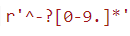
\includegraphics[width=0.2\linewidth]{images/AdminPanel/regexInputFormatter.png}
            \caption{Regular expression for input validation}
        \end{figure}
                
        \item A \texttt{TextInputFormatter} prevents multiple decimal points in a single number. If a user attempts to insert a second decimal point, the input is automatically rejected.
        
        \item The last \texttt{TextInputFormatter} ensures the number of digits before the decimal point is limited to a maximum of 3. Additionally, the value before the decimal point must not exceed 180.
    \end{itemize}
\newpage


\subsubsection{Additional Functionalities}
    This section highlights various functionalities implemented to improve the overall usability of the application. These additions are designed to support administrative tasks and ensure a seamless user experience.

\paragraph{Notification}
\label{fig:Notification}

    To inform the administrator about the success or failure of an operation, a \texttt{Notification} is displayed on the bottom left, overlaying the \texttt{AdminMapComponent}. This notification appears when:

    \begin{itemize}
        \item An address is added, edited, or deleted.
        \item Validation fails.
        \item Coordinates are selected on the \texttt{AdminMapComponent} (\ref{fig:Select Coordinates on Map}).
        \end{itemize}


\begin{figure}[H]
    \centering
    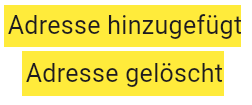
\includegraphics[width=0.4\linewidth]{images/AdminPanel/NotificationExamples.png}
    \caption{Notification examples}
\end{figure}

To display this notification, the \texttt{showNotification} method is called. This method sets the \texttt{notificationVisible} variable to \texttt{true} and starts a \texttt{Timer} to turn it set it back to \texttt{false} three seconds later, so it goes away in a short time. This method accepts a message as a parameter, which is saved in the \texttt{notificationText} variable.
\lstset{style=mycsharp, caption=showNotification method}
\begin{lstlisting}
    void showNotification(String message) {
    setState(() {
      notificationText = message;
      notificationVisible = true;
    }); 
    Timer(Duration(seconds: 5), () {
      setState(() {
        notificationVisible = false;
      });
    });
  }
\end{lstlisting}

When the \texttt{notificationVisible} variable is set to \texttt{true}, the UI-component which shows the notification is rendered.
\lstset{style=mycsharp, caption=Notification in AddressPage}
\begin{lstlisting}
    Positioned(
        left: 10,
        bottom: 10,
        child: (notificationVisible)
            ? Container(
                padding: EdgeInsets.all(4),
                color: Colors.yellow,
                child: Text(
                    notificationText,
                    style: TextStyle(fontSize: 20),
                ),
                )
            : Container(),
        ),
\end{lstlisting}

\subsubsection{Edit multiple addresses}
\label{fig:Edit multiple addresses}
To make it easier to edit mulitple addresses at once, the CTRL-Button on the keyboard is listened to. When the CTRL-Button is pressed, the \texttt{isCtrlPressed} variable is set to \texttt{true}. This variable is passet to the \texttt{DatabaseViewComponent} and the \texttt{AdminMapComponent}, to inform them that multiple addresses want to be selected. The components can use the, as a parameter given, \texttt{markerSelected} function to set the selected addresses in the \texttt{AddressPage}. The \texttt{saveAddress} method is called to save multiple addresses.\\



To listen to the CTRL-Button, the predefined \texttt{RawKeyboardListener} is used. This widget sets the \texttt{isCtrlPressed} variable to \texttt{true} when the CTRL-Button is pressed and to \texttt{false} when it is released. to make sure that repeadetly pressing the CTRL-Button, which happens if the button is pressed and held, does not interfere with the \texttt{isCtrlPressed} variable, the condition \texttt{event.repeat == false} is used.

\lstset{style=mycsharp, caption=RawKeyboardListener in AddressPage}
\begin{lstlisting}
    RawKeyboardListener(
        autofocus: true,
        focusNode: FocusNode(),
          onKey: (event) {
          if ((event.isKeyPressed(LogicalKeyboardKey.controlLeft) ||
               event.isKeyPressed(LogicalKeyboardKey.control) || 
               event.isKeyPressed(LogicalKeyboardKey.controlRight)) && event.repeat == false) {
              setState(() {
                isCtrlPressed = true;
              });
          } else if (event is RawKeyUpEvent && event.logicalKey == LogicalKeyboardKey.controlLeft) {
              setState(() {
                isCtrlPressed = false;
              });
          }
        },
    ),
\end{lstlisting}


The \texttt{markerSelected} method also updates the \texttt{InputField} for the house number by listing the house numbers of the selected addresses in the controller.

\lstset{style=mycsharp, caption=Listed house numbers for multiple selected addresses}
\begin{lstlisting}
    controllers["houseNumber"]?.text = selectedAddresses
              .map((address) => address.houseNumber)
              .toList()
              .join(', ');
\end{lstlisting}

The \texttt{InputField} looks like this:
\begin{figure}[H]
    \centering
    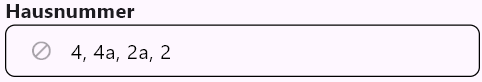
\includegraphics[width=0.6\linewidth]{images/AdminPanel/listedHouseNumbersInputField.png}
    \caption{House numbers of multiple selected addresses}
\end{figure}

The selected addresses are saved in the \texttt{selectedAddresses} variable in the \texttt{AddressPage}. If multiple addresses are selected, certain \texttt{InputFields} such as house numbers, coordinates, or comments will be disabled because changing them for all selected addresses would not make sense. This can be achieved by setting the \texttt{editable} parameter of these \texttt{InputFields} to \texttt{selectedAddresses.length <= 1}, so that they are only editable when a single address is selected.

\subsubsection{Edit all Addresses from a Street}
All addresses from a street can be edited at once. This is almost the same as editing multiple addresses (\ref{fig:Edit multiple addresses}), but instead of selecting the addresses by clicking on them, a street is selected. When a street is selected, all its addresses are selected. A street can be selected in two ways:

\paragraph{Select Street via AdminMapComponent}
Every click on the \texttt{AdminMapComponent} is checked if it is near a street. Because there is no predefined method to check if a point is on a street, the \texttt{isPointNearPolyline} method was implemented. This method checks if the click was on the street. More information about this method can be found in the \texttt{AdminMapComponent} section \ref{fig:AdminMapComponent}.\\

\paragraph{Select Street via Button}
This was implemented because we encountered a problem where it was not possible to click on a street on some devices. To ensure that this feature is usable on all devices, a dropdown button to choose a street and a button to select it were implemented.\\

\begin{figure}[H]
    \centering
    \includegraphics[width=0.6\linewidth]{images/AdminPanel/SelectStreetButton.png}
    \caption{Button to select a street}
\end{figure}


\subsubsection{Edit Odd / Even Streets}
One requirement was that addresses from one street could be automatically added to two areas based on whether the house number is even or odd. This is because it is common for all addresses with even house numbers to be on one side of the street and those with odd house numbers on the other side. This way, it is easier to assign the street sides to different areas, so that "Sternsinger" participants don't have to cross the street so often.\\\\
To make this possible, the administrator has to select a street in the \texttt{AdminMapComponent}(\ref{fig:Select Street}), then a blue button beneath the \texttt{InputFields} appears. \\

\begin{figure}[H]
    \centering
    
\includegraphics[width=0.7\linewidth]{images/AdminPanel/splitStreetButton.png}
    \caption{Button to split street}
\end{figure}

\begin{figure}[H] 
    \begin{minipage}{0.6\textwidth}
        After pressing this button, a dialog appears, where the administrator can select the areas for the addresses with even and odd house numbers.
    \end{minipage}
    \hfill
    \begin{minipage}{0.35\textwidth}
        \centering
        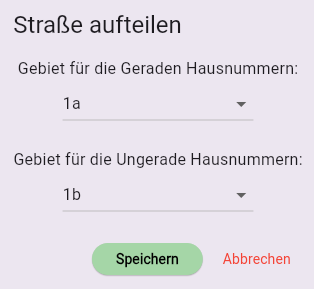
\includegraphics[width=\linewidth]{images/AdminPanel/splitStreetDialog.png}
        \caption{Dialog to split street}
    \end{minipage}
\end{figure}


The "Speichern" button triggers the \texttt{AdminAddressProvider} and shows a \texttt{Notification}(\ref{fig:Notification}) if the operation was successful or not. After that, the dialog is closed.

\lstset{style=mycsharp, caption=onPressed save button in splitStreetDialog}
\begin{lstlisting}
    int resultCode = await addressProvider.putAddressesOddEven(selectedAddresses.first.street.name, selectedAddresses.first.street.postalCode, selectedAreaEven, selectedAreaOdd);
    if (resultCode == 200) {
        showNotification("Adressen gespeichert", () => showAddressSavedNotification = true);
    } else {
        showNotification("Fehler beim Speichern", () => showAddAddressNotification = true);
    }
    if (!context.mounted) return;
    Navigator.of(context).pop();
\end{lstlisting}


\begin{figure}[H]
    \setstretch{1.5} % Erhöht den Zeilenabstand
    \centering
    \begin{minipage}{0.55\textwidth} % Linke Seite für den Text
        \subsubsection{Filter}
        With the Filter field, the administrator can filter the addresses displayed. It contains three dropdown menus to set the filter criteria, with one checkbox for each to toggle them. These filters can be combined as desired. 
    \end{minipage}
    \hfill 
    \begin{minipage}{0.4\textwidth} % Rechte Seite für das Bild
        \centering
        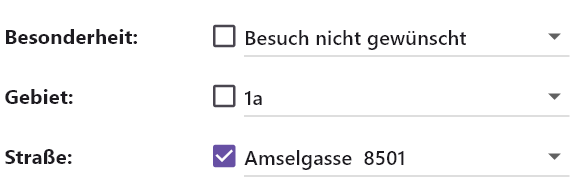
\includegraphics[width=\linewidth]{images/AdminPanel/FilterField.png}
        \caption{Filter field in AddressPage}
        \label{fig:adminpanel_filter}
    \end{minipage}
\end{figure}

The filter is passed and applied to the \texttt{AdminMapComponent} and the \texttt{DatabaseViewComponent}. The criteria and their enabled/disabled state are managed by the following variables in the \texttt{AddressPage} class.
\lstset{style=mycsharp, caption=Filter variables in AddressPage}
\begin{lstlisting}
    bool specialFeatureFilter = false;
    bool areaFilter = false;
    bool streetFilter = false;
    
    String selectedStreetFilter = "";
    String selectedSpecialFeatureFilter = "";
    String selectedAreaFilter = "";
\end{lstlisting}

This is an example of how a \texttt{FilterRow} is defined in the \texttt{AddressPage} class (\ref{fig:FilterRow}):
\lstset{style=mycsharp, caption=FilterRow in AddressPage}
\begin{lstlisting}
    FilterRow(
        label: "Besonderheit:",
        tooltipMessage: "Besonderheitsfilter aktivieren/deaktivieren",
        filterValue: specialFeatureFilter,
        onFilterChanged: (bool? newValue) {
          setState(() => specialFeatureFilter = newValue ?? false);
        },
        selectedValue: selectedSpecialFeatureFilter,
        items: specialFeatureTextList,
        onDropdownChanged: (String? newValue) {
          setState(() => selectedSpecialFeatureFilter = newValue ?? "");
        },
      ),
\end{lstlisting}


 

\subsection{ListEditPage}
The \texttt{ListEditPage} is used to manage \textbf{streets}, \textbf{special features}, and \textbf{areas}. It allows the administrator to add, edit, and delete these entities. The page is divided into two parts. On the right side, all entities are displayed in a table and can be selected. On the left, there is a dropdown menu for selecting between the three options. The information of the selected item is shown in \texttt{InputFields} on the this side, where the information can be edited, saved or deleted using the "Speichern" or the "Löschen" button.

\begin{figure}[H]
    \centering
    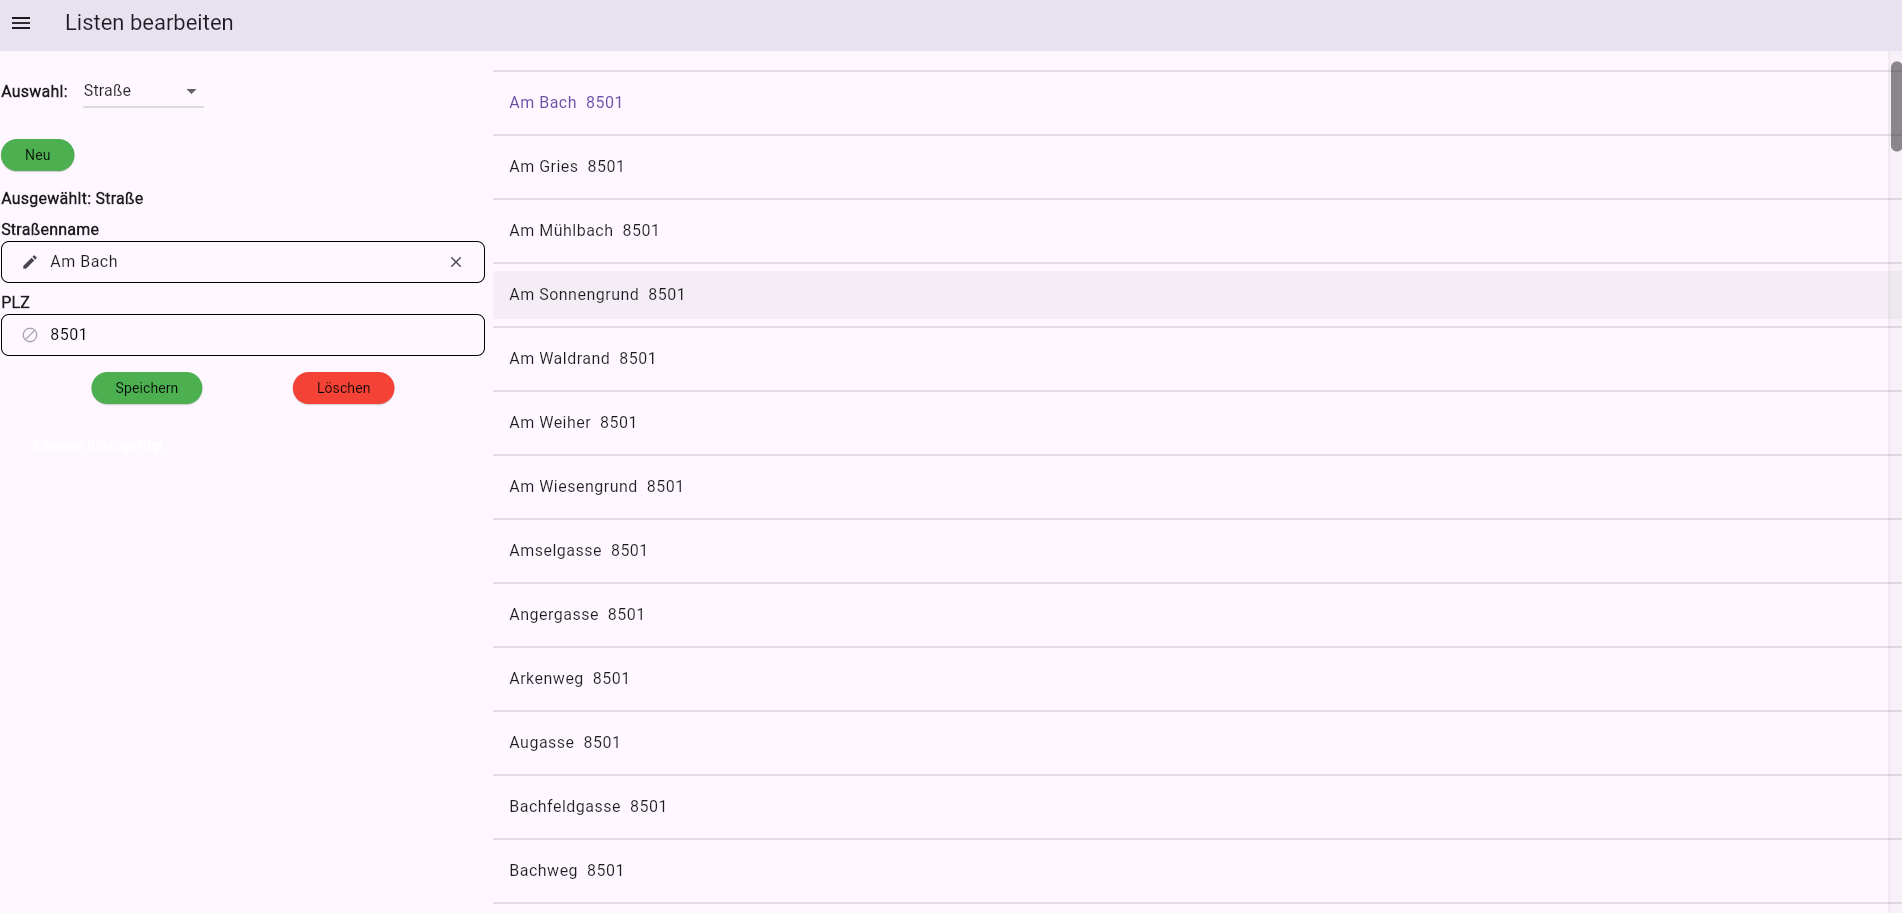
\includegraphics[width=0.9\linewidth]{images/AdminPanel/ListEditPage.png}
    \caption{ListEditPage}
\end{figure}

\subsubsection{QR-Code Visualization for Areas}
To make it easier for users of the user application to get information about their area, a QR-Code is generated for every area, which can be scanned to get all information. The QR-Code contains the name of the area. The currently selected area is saved in the \texttt{selectedItem} variable.

\begin{figure}[H]
    \centering
    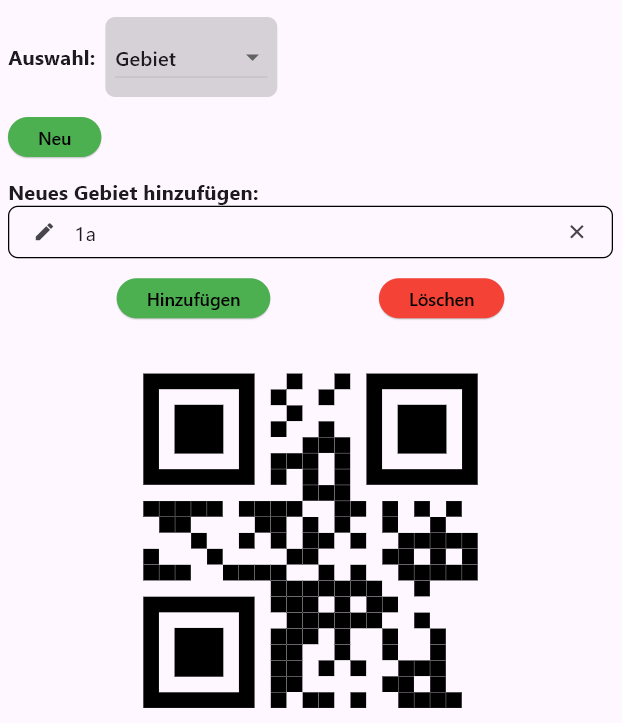
\includegraphics[width=0.4\linewidth]{images/AdminPanel/QrImageView.png}
    \caption{QR-Code for area}
\end{figure}

To display the QR-Code, the \texttt{QrImageView} Widget is used. 

\lstset{style=mycsharp, caption=QrCode Generation in ListEditPage}
\begin{lstlisting}
    QrImageView(
        data: selectedItem,
        size: 300,
        padding: const EdgeInsets.all(16.0),
        gapless: false,
        ),
\end{lstlisting}

\subsubsection{QR-Code-PDF Download}
A PDF with all QR-Codes for all areas can be downloaded, making it easier to distribute the information to users. The PDF is generated with the \texttt{savePDF} method of the \texttt{PDFSaver} class.

A QR-Code is generated with the \texttt{generateQRCode} method in the \texttt{ListEditPage} class. This method takes a string as the parameter and converts this string to a QR-Code using the predefined \texttt{QrPainter}, which helps with painting a QR-Code \autocite{pub.dev/QrPainter-class}. The method then generates an image of the QR code with this class, converts this into byte data in PNG format, and finally transforms the byte data into a list of bytes (Uint8List) that can be used to display the QR-code in the pdf.\\

The savePdf method generates a PDF document containing QR-codes for all areas. It uses the predefined pdf package, imported as pw, to create and manage the PDF \autocite{pub.dev/pdf}. The function starts by initializing a new PDF using the pw.Document() class and an empty list to store the generated QR codes. It then iterates over a list of areas, generating a QR code for each area's description using the \texttt{generateQRCode} method and adding it to the list.\\

After that, a page is added to the PDF document using the pw.MultiPage widget, which includes a title and every description of all areas with their corresponding QR-codes. After building the page content, the PDF data is saved to a variable by calling pdf.save(). Finally, the PdfSaver.savePdf method is called with the data to save it to a PDF named "Gebiete.pdf".



\todo{QR-Code PDF Download Foto einfügen}




\subsection{Components}

\subsubsection{AdminMapComponent}
\label{fig:AdminMapComponent}
With this component, the addresses can be displayed on a geographic map. The map used is the OpenStreetMap which if free to use for everyone. Even though the Admin Panel is not used commercially, OpenStreetMap's attribution rules are followed. The map shows the required copyright notice "© OpenStreetMap contributors" in the bottom-left corner. The word "OpenStreetMap" is clickable and links directly to https://www.openstreetmap.org/copyright, opening the official license page in a new tab. This meets OpenStreetMap's license requirements by clearly acknowledging the data source and linking to their terms. \autocite{OpenStreetMap}
\begin{figure}[H]
    \centering
    
\includegraphics[width=0.2\linewidth]{images/AdminPanel/Openstreetmapverweis.png}
    \caption{OpenStreetMap attribution}
\end{figure}




\paragraph{Select Street}
\label{fig:Select Street}

To select a street, the \texttt{isPointNearPolyline} method was implemented. This method checks if the click was on a street. As parameters, it takes the coordinates of the click as a \texttt{LatLng} object and a street as a list of \texttt{LatLngs}. After each click on the map, a loop is triggered that calls the \texttt{isPointNearPolyline} method for every street, passing the click coordinates during each iteration.\\

The \texttt{isPointNearPolyline} uses another loop, which iterates over all points of the street. Because the street is represented as a list of \texttt{LatLngs}, every two points are connected to form a line. Every iteration of the loop a helper method \texttt{isNear} is called, which calculates the distance between the click and the currently iterated line segment. 

\lstset{style=mycsharp, caption=isPointNearPolyline method}
\begin{lstlisting}
  bool isPointNearPolyline(LatLng point, List<LatLng> polylinePoints) {
    const double tolerance = 0.00005;
    for (int i = 0; i < polylinePoints.length - 1; i++) {
       if (_isNear(point, polylinePoints[i], polylinePoints[i + 1], tolerance)) {
        return true;
      }
    }
    return false;
  }
\end{lstlisting}

The \texttt{isNear} method takes the click point, the two points for the line and the tolerance. If the distance is smaller than the predefined tolerance, the method returns \texttt{true}, indicating that the click was on the street.

\lstset{style=mycsharp, caption=isNear method}
\begin{lstlisting}
    bool _isNear(LatLng p, LatLng a, LatLng b, double tolerance) {
        double dx = b.latitude - a.latitude;
        double dy = b.longitude - a.longitude;
        double t = ((p.latitude - a.latitude) * dx + (p.longitude - a.longitude) * dy) / (dx * dx + dy * dy); 
        t = t.clamp(0, 1);
        double cx = a.latitude + t * dx;
        double cy = a.longitude + t * dy;
        return (p.latitude - cx).abs() + (p.longitude - cy).abs() <= tolerance;
    }
\end{lstlisting}


\paragraph{onClickNewAddress}

\paragraph{Select Coordinates on Map}
\label{fig:Select Coordinates on Map}

\subsubsection{DatabaseViewComponent}
\label{fig:DatabaseViewComponent}
To display the addresses in a table, this component is used. As parameters it takes the \texttt{selectedAddresses}, the filter variables aswell as the \texttt{isCtrlPressed} variable from the \texttt{AddressPage}, which is used to track if mulitple addresses want to be selected. The \texttt{selectedAddresses} are displayed in the table and can be selected by clicking on them. \\

On the top are two fields 

\subsubsection{PDFSaver}
The \texttt{PdfSaver} class provides a static method to save a PDF file from a byte array. The method \texttt{savePdf} takes a Uint8List of bytes and a String representing the file name as parameters. Depending on the platform, it saves the PDF file accordingly.\\


\lstset{style=mycsharp, caption=savePdf method in PDFSaver}
\begin{lstlisting}
    static Future<void> savePdf(Uint8List bytes, String fileName) async {
        if (kIsWeb) {
            final blob = html.Blob([bytes], 'application/pdf');
            final url = html.Url.createObjectUrlFromBlob(blob);
            final anchor = html.AnchorElement(href: url)
                ..target = 'blank'
                ..download = fileName
                ..click();
            html.Url.revokeObjectUrl(url);
        } else {
            await FileSaver.instance.saveFile(
                name: fileName,
                bytes: bytes,
                ext: 'pdf',
                mimeType: MimeType.pdf,
            );
        }
    }
    
\end{lstlisting}
  \subsubsection{AdminAddressProvider}
This class serves as a bridge between the Admin Panel and the backend. It is responsible for all CRUD operations on addresses, streets, special features, and areas. It is used in the \texttt{AddressPage} and the \texttt{ListEditPage}. 

The \texttt{AdminAddressProvider} includes the \texttt{ChangeNotifier} mixin. A mixin is a way to reuse code across mulitple classes, without using inheritance like in Java.\autocite{dart.dev} The \texttt{ChangeNotifier} mixin is used to notify the UI when the data changes. \autocite{flutter.dev} This is done by calling the \texttt{notifyListeners} method.\\

Here is a typical method in the \texttt{AdminAddressProvider} class. It contains these functionalities:

\begin{itemize}
    \item \texttt{async}: enables non-blocking operations and ensures that the UI remains responsive while waiting for tasks like network requests to complete.
    \item \texttt{await http.get}: sends a GET request to the server to fetch all streets and waits for the response.
    \item \texttt{jsonDecode}: processes the JSON response from the server.
    \item \texttt{utf8.decode}: transforms the UTF-8 encoded response body into readable text.
    \item \texttt{map}: converts the decoded JSON to a list of \texttt{Street} objects.
    \item \texttt{sort}: sorts the list alphabetically.
    \item \texttt{notifyListeners}: notifies the listeners that the data has changed.
    \item \texttt{catch}: catches any errors that occur during the operation.
\end{itemize}
\lstset{style=mycsharp, caption=typical method in AdminAddressProvider}
\begin{lstlisting}
    Future<void> fetchStreets() async {
      try {
        final response = await http.get(Uri.parse('$serverURL/$baseURL/admin/getAllStreets'));
        if (response.statusCode == 200) {
          final List<dynamic> decodedJSON = jsonDecode(utf8.decode(response.bodyBytes));
          streets = decodedJSON.map((json) => Street.fromJson(json)).toList();
          streets.sort((a, b) => a.name.compareTo(b.name));
          notifyListeners();
        } else {
          throw Exception('Failed to load streets');
        }
      } catch (e) {
        print('Error fetching streets: $e');
      }
    }
\end{lstlisting}

\subsubsection{CustomHttpClient}

\subsection{Models}

\subsubsection{AreaWithBorder}

\subsubsection{ScreenItem}

\subsection{Widgets}

\subsubsection{InputField}
\label{fig:InputField} 
This widget defines a customizable input field. The \texttt{InputField} requires a label and a \texttt{TextEditingController} for managing the input. Optional parameters include a boolean \texttt{editable}, a list of \texttt{Strings} called \texttt{dropDownOptions} and a boolean \texttt{isCoordinateInput} to specify if the input should be numeric.\\

To display if the \texttt{InputField} is editable, icons are displayed on the left side of the field. If the field is not editable, the icon is a blocked symbol, and if it is editable, a pencil is displayed. When the \texttt{InputField} is editable and it is not a dropdown, a cross is displayed on the right side. When it is pressed, the content is cleared.\\

\begin{figure}[H]
    \centering
    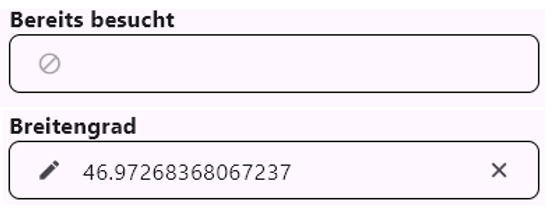
\includegraphics[width=0.4\linewidth]{images/AdminPanel/InputFieldExamples.png}
    \caption{InputField examples}
\end{figure}

If the dropDownOptions parameter is provided with a non-empty list of strings, the input field renders as a dropdown menu. The selected value is displayed, and users can choose from the provided options. The dropdown value is automatically synced with the TextEditingController.\\

To guarantee valid inputs, the \texttt{InputField} uses an \texttt{inputFormatter} to validate the input. This formatter is only applied when the \texttt{isNumberInput} parameter is set to true. For further information about the validation, see \ref{fig:InputField Coordinates Validation}.


\subsubsection{FilterRow}
\label{fig:FilterRow}

This widget defines a reusable filter row. The \texttt{FilterRow} combines a label, a toggleable checkbox, and a dropdown menu to enable dynamic data filtering. It requires several parameters:
\begin{itemize}
    \item \texttt{label}: A string for identifying the filter.
    \item \texttt{tooltipMessage}: A message to display when hovering over the checkbox.
    \item \texttt{filterValue}: A boolean to track the filter's active state.
    \item \texttt{items}: A list of strings for the dropdown options.
    \item \texttt{selectedValue}: Manages the selected dropdown value.
    \item \texttt{onFilterChanged}: A callback for updating the filter state. 
    \item \texttt{onDropdownChanged}: A callback for updating the selected dropdown value.
\end{itemize}


\begin{figure}[H]
    \centering
    
\includegraphics[width=0.5\linewidth]{images/AdminPanel/FilterRow.png}
    \caption{FilterRow}
\end{figure}

